\documentclass{article}

\usepackage{siunitx} % Provides the \SI{}{} and \si{} command for typesetting SI units
\usepackage{graphicx} % Required for the inclusion of images
\usepackage{amsmath} % Required for some math elements 
\usepackage[export]{adjustbox} % loads also graphicx
\usepackage{listings}
\usepackage{matlab-prettifier}
\usepackage{float}
\usepackage[most]{tcolorbox}
\usepackage{amsfonts}
\usepackage{color}
\usepackage{titlesec}
\usepackage{caption}
\usepackage{subcaption}

\newcommand{\R}{\mathbb{R}}

\usepackage{xcolor}

\DeclareCaptionFont{white}{\color{white}}
\DeclareCaptionFormat{listing}{%
  \parbox{\textwidth}{\colorbox{gray}{\parbox{\textwidth}{#1#2#3}}\vskip-4pt}}
\captionsetup[lstlisting]{format=listing,labelfont=white,textfont=white}
\lstset{frame=lrb,xleftmargin=\fboxsep,xrightmargin=-\fboxsep}
\titleformat{\section}[runin]
  {\normalfont\Large\bfseries}{\thesection}{1em}{}
\titleformat{\subsection}[runin]
  {\normalfont\large\bfseries}{\thesubsection}{1em}{}


\setlength\parindent{0pt} % Removes all indentation from paragraphs

\renewcommand{\labelenumi}{\alph{enumi}.} % Make numbering in the enumerate environment by letter rather than number (e.g. section 6)

%\usepackage{times} % Uncomment to use the Times New Roman font

%----------------------------------------------------------------------------------------
%	DOCUMENT INFORMATION
%----------------------------------------------------------------------------------------

\title{AMATH 353: Homework 10 \\Due May, 8 2018 \\ ID: 1064712} % Title

\author{Trent \textsc{Yarosevich}} % Author name

\date{\today} % Date for the report

\begin{document}
\maketitle % Insert the title, author and date
\setlength\parindent{1cm}

\begin{center}
\begin{tabular}{l r}
%Date Performed: December 1, 2017 \\ % Date the experiment was performed
Instructor: Jeremy Upsal % Instructor/supervisor
\end{tabular}
\end{center}

% If you wish to include an abstract, uncomment the lines below
% \begin{abstract}
% Abstract text
% \end{abstract}

%----------------------------------------------------------------------------------------
%	SECTION 1
%----------------------------------------------------------------------------------------
\section*{Part 1}
We consider the heat equation and the following IBVP:
\begin{align*}
&u_t=4u_{xx} & 0<&x<1, & t&> 0\\
&u(0, t)= u_x(1, t) = 0 && & t&> 0\\
&u(x,0)= x(1-x). && &&
\end{align*}
I've used separation of variables in the same fashion as I did in HW 8, which is to say I put the $k$ term with the $x$ equation. Using $k = 4$ this results in:
\begin{equation}
\begin{aligned}
G'(t) = \lambda G(t)\\
F''(x) = \frac{\lambda}{4}F(x)
\end{aligned}
\end{equation}
As in HW 8, the only allowed $\lambda$ values with this setup were $\lambda < 0$, which resulted in the following using the characteristic polynomial and Euler's Formula, and $\lambda = -r^2, r \in \mathbb{R}^+$:
\begin{equation}
F(x) = C_1\cos(\frac{r}{2}x) + C_2\sin(\frac{r}{2}x)
\end{equation}
We then apply the BCs to this:
\begin{equation}
\begin{aligned}
F(0) = C_1\cos(0) + C_2\sin(0) = 0\\
C_1 = 0\\
F'(x) = \frac{r}{2}C_2\cos(\frac{r}{2}x)\\
F'(1) = \frac{r}{2}C_2\cos(\frac{r}{2}) = 0
\end{aligned}
\end{equation}
Thus without setting $C_2 = 0$ the BC is only satisfied when $\cos(\frac{r}{2}) = 0$, which means the argument is equal to odd integer multiples of $\frac{\pi}{2}$:
\begin{equation}
\begin{aligned}
n \in \mathbb{Z}^+\\
\frac{r}{2} = \frac{\pi (2n-1)}{2}\\
r = \pi (2n-1)\\
\lambda_n = - ( \pi(2n-1))^2\\
\end{aligned}
\end{equation}
\begin{tcolorbox}[minipage,colback=white,arc=0pt,outer arc=0pt]
\begin{equation}
F_n(x) = C_2\sin(\frac{\pi(2n-1)}{2}x)
\end{equation}
\end{tcolorbox}
Turning to the equation $G'(t) = \lambda G(t)$, we can simply solve with separation of variables (ODE 101 version):
\begin{equation}
\begin{aligned}
\int \frac{dG}{dt} = \int \lambda G(t)\\
ln(G(t)) = \lambda t + C\\
G(t) = Ae^{\lambda t}
\end{aligned}
\end{equation}
Combining the above with the result in equation (4) and substituting $\lambda_n$, we get a solution for $u$, and note I have consolidated the product of the arbitrary constants in a single new arbitrary constant. Consequently, we can also use superposition to rewrite the equation as a sum of solutions.
\begin{tcolorbox}[minipage,colback=white,arc=0pt,outer arc=0pt]
\begin{equation}
\begin{aligned}
u_n(x, t) = Ae^{\lambda_n t}\sin(\frac{\pi(2n-1)}{2}x)\\
u(x, t) = \sum_{n=1}^{\infty} A_ne^{\lambda_n t}\sin(\frac{\pi(2n-1)}{2}x)
\end{aligned}
\end{equation}
\end{tcolorbox}
We now have to match this form to the initial condition $u(x, 0) = x(1-x)$, which gives us the following equation. Let this IC be $f(x)$:
\begin{equation}
\begin{aligned}
u(x, 0) = \sum_{n=1}^{\infty} A_ne^{\lambda_n (0)}\sin(\frac{\pi(2n-1)}{2}x) = f(x)\\ 
f(x) = \sum_{n=1}^{\infty} A_n\sin(\frac{\pi(2n-1)}{2}x)
\end{aligned}
\end{equation}
This gives us the Fourier Series form of the initial condition. Because we need to make use of the orthogonality relations, and $f(x)$ is only defined from $x \in [0, 1]$, we will use the odd extension of $f(x)$ because the BCs specify a fixed point at the origin. And indeed, using the even extension in this situation just results in a $0$ constant anyway.\\
\\
We define the odd extension as follows:
\begin{equation}
f(x) = x(1-x)
\end{equation}
\[f_o(x)=
  \begin{cases}
			f(x), \; \; \; x \geq 0 \\
			-f(-x), \; \; \; x < 0
            \end{cases}
\]
As stated in the homework, $A_0 = 0$ because $\int_0^1 x(1-x) = 0$. For our one constant $A_n$ we then have the following:
\begin{equation}
\begin{aligned}
L = 1\\
A_n = \int_{-1}^1 f_o(x)\sin(\frac{\pi(2n-1)}{2}x)
\end{aligned}
\end{equation}
Because both $f_o(x)$ and $\sin$ are odd, the resulting function is even, and because $f_o(x) = f(x)$ for all $x \geq 0$ we have the following:
\begin{equation}
\begin{aligned}
\int_{-1}^1 f_o(x)\sin(\frac{\pi(2n-1)}{2}x) = 2\int_0^1 f_o(x)\sin(\frac{\pi(2n-1)}{2}x)\\
2\int_0^1 f_o(x)\sin(\frac{\pi(2n-1)}{2}x) = 2\int_0^1 f(x)\sin(\frac{\pi(2n-1)}{2}x)\end{aligned}
\end{equation}
We now solve this integral using integrating factors:
\begin{equation}
\begin{aligned}
A_n = 2\int_0^1 f(x)\sin(\frac{\pi(2n-1)}{2}x)\\
u = x(1-x), \; \; du = (1-2x)dx\\
dv = \sin(\frac{\pi(2n-1)}{2}x)\\
v = \int dv = \frac{-2}{\pi(2n-1)}\cos(\frac{\pi(2n-1)}{2}x)\\
\int udv = \frac{-2x + 2x^2}{\pi(2n-1)}\cos(\frac{\pi(2n-1)}{2}x) - \int \frac{-2 + 4x}{\pi(2n-1)}\cos(\frac{\pi(2n-1)}{2}x)dx
\end{aligned}
\end{equation}
We then continue to solve $\int vdu$ using integrating factors again:
\begin{equation}
\begin{aligned}
\int \frac{-2 + 4x}{\pi(2n-1)}\cos(\frac{\pi(2n-1)}{2}x)dx\\
u = \frac{-2 + 4x}{\pi(2n-1)}\\
du = \frac{4}{\pi(2n-1)}dx\\
dv = \cos(\frac{\pi(2n-1)}{2}x)\\
v = \frac{2}{\pi(2n-1)}\sin(\frac{\pi(2n-1)}{2}x)\\
\int udv = \frac{-4 + 8x}{\pi^2(2n-1)^2}\sin(\frac{\pi(2n-1)}{2}x) - \int \frac{8}{\pi^2(2n-1)^2)}\sin(\frac{\pi(2n-1)}{2}x)\\
= \frac{-4 + 8x}{\pi^2(2n-1)^2}\sin(\frac{\pi(2n-1)}{2}x) + \frac{16}{\pi^3(2n-1)^3}\cos(\frac{\pi(2n-1)}{2}x)
\end{aligned}
\end{equation}
Then substituting this result into the original integral, and consolidating the numerators, we get:
\begin{equation}
A_n  = \Big[ \frac{(-2x + 2x^2)(\pi^2(2n-1)^2) - 16)\cos(\frac{\pi(2n-1)}{2}x) + (4-8x)\pi(2n-1)\sin(\frac{\pi(2n-1)}{2}x)}{\pi^3(2n-1)^3} \Big] \Big|_0^1
\end{equation}
Letting the denominator be some constant $c$ for a moment, we have
\begin{multline}
A_n c = (0)(\pi^2(2n-1)^2) - 16)\cos(\frac{\pi(2n-1)}{2}) + (-4)\pi(2n-1)\sin(\frac{\pi(2n-1)}{2}) \\ - (0)(\pi^2(2n-1)^2) - 16)\cos(0) + (4)\pi(2n-1)\sin(0)
\end{multline}
Simplifying this and moving the  denominator back over, we have:
\begin{equation}
A_n = \frac{-16\cos(\frac{\pi(2n-1)}{2}) - 4\pi(2n-1)\sin(\frac{\pi(2n-1)}{2}) + 16}{\pi^3(2n-1)^3}
\end{equation}~\\
\\
At this point we can make a few observations. For $n \in \mathbb{Z}^+$, we can see that $\cos(\frac{\pi(2n-1)}{2}) = 0$. Further we can observe that $\sin(\frac{\pi(2n-1)}{2}) = (-1)^{n+1} = -(-1)^n$. Substituting these in and multiplying the entire result of the integral we solved by $2$, we get the final value for $A_n$, and so we can give the complete solution for $u(x,t)$ that matches our IC at $u(x,0)$:
\begin{tcolorbox}[minipage,colback=white,arc=0pt,outer arc=0pt]
\begin{equation}
\begin{aligned}
\lambda_n = - ( \pi(2n-1))^2\\
A_n = \frac{8\pi(2n-1)(-1)^n + 16}{\pi^3(2n-1)^3}\\
u(x, t) = \sum_{n=1}^{\infty} A_ne^{\lambda_n t}\sin(\frac{\pi(2n-1)}{2}x)
\end{aligned}
\end{equation}
\end{tcolorbox}
\section*{Part 2}
We can see that that as $t \to \infty$, the $e^{\lambda t}$ term gets very small, regardless of the number of modes. Indeed, it gets small more quickly for higher modes, which I would speculate is a mathematical result of the larger number of oscillations experiencing greater friction due to their higher overall arc length (just a guess?). This is what we'd expect from the heat equation, since over time all the heat dissipates through the rod, or whatever else it is we're modeling. \\
\\
Here is a solution surface showing this behavior:
\begin{figure}[H]
  \centering
    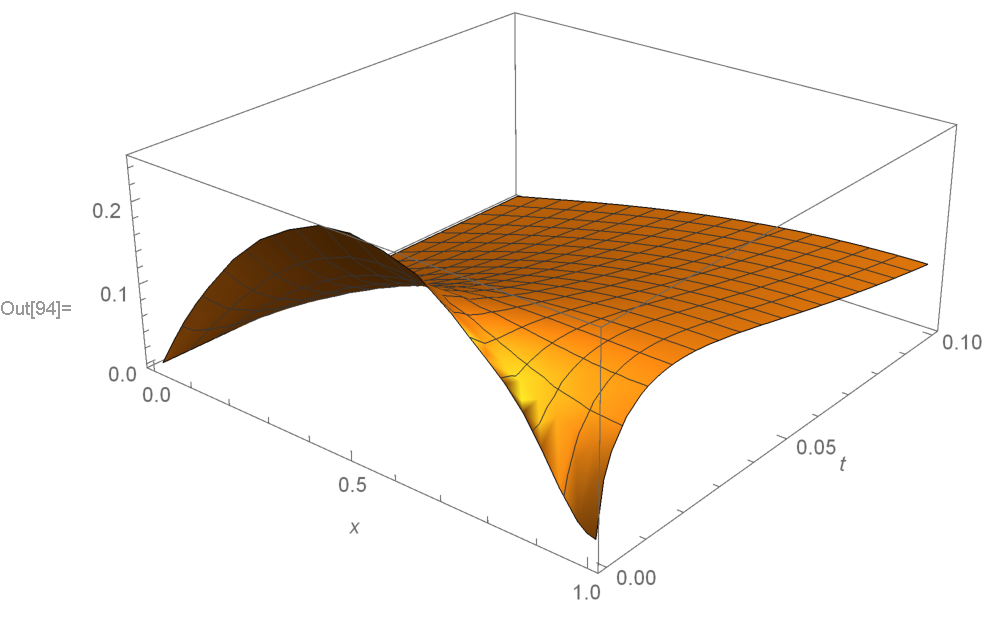
\includegraphics[width=\textwidth]{part2_plot.pdf}
    \caption{$u(x,t), t \in [0,.1], N = 10$}
\end{figure}
\noindent Also notice that in the initial condition, at the $x$ values in which the concavity is positive, the solution surface actually increases until the $e^{\lambda t}$ term becomes sufficiently small. This is also to be expected since the time velocity of the heat equation is directly related to the spatial acceleration. Furthermore we can see that the BC $u_x(1, t) = 0$ isn't satisfied in the solution surface. I think this is because the initial condition results in $u(1, 0)$ having non-zero concavity.
\section*{Part 3}
We have the following piecewise function, \textit{which we can easily see is an even function.}:
\[f(x)=
  \begin{cases}
			0, \; \; \; x \in [-\pi, \frac{-\pi}{2}] \\
			1, \; \; \; x \in [\frac{-\pi}{2} , \frac{\pi}{2}\\
			0, \; \; \; x \in [\frac{\pi}{2}, \pi] \\
            \end{cases}
\]
Which is represented with a Fourier Series of the form, with $L = \pi$:
\begin{equation}
f(x) = A + \sum_{n=1}^{\infty} A_n\cos(nx) + B_n\sin(nx)
\end{equation}
Using this we can use the standard relations described in the lecture notes and in class to determine the coefficients.
\begin{equation}
A = \frac{1}{2\pi} \int_{-\pi}^{\pi}f(x)dx = \frac{1}{\pi}\int_0^{\pi}f(x)dx
\end{equation}
We then define this integral as a sum of the integrals for each part of the piecwise function, but it is clear that the integral for $x\in [\frac{\pi}{2}, \pi]$ is zero. The remaining integral is quite simple because it is a slope of zero:
\begin{equation}
\begin{aligned}
\frac{1}{\pi}\int_0^{\frac{\pi}{2}}f(x)dx = \frac{1}{2}\\
A = \frac{1}{2}
\end{aligned}
\end{equation}
Because $f(x)$ is an even function, $B_n = 0$ because the result is an integral of an odd function across a symmetric domain containing the origin. More intuitvely, just looking at this function, it seems obvious that a cosine basis would be used to define it with a Fourier Series. Thus, because both cosine and $f(x)$ are even functions, their product is even, giving the following:
\begin{equation}
A_n = \frac{1}{\pi} \int_{-\pi}^{\pi}f(x)\cos(nx)dx = \frac{2}{\pi}\int_0^{\pi}f(x)\cos(nx)dx
\end{equation}
Let us consider $g(x) = f(x)\cos(nx)$. This would give the following piecewise function:
\[g(x)=
  \begin{cases}
			0, \; \; \; x \in [-\pi, \frac{-\pi}{2}] \\
			cos(nx), \; \; \; x \in [\frac{-\pi}{2} , \frac{\pi}{2}\\
			0, \; \; \; x \in [\frac{\pi}{2}, \pi] \\
            \end{cases}
\]
Thus we have:
\begin{equation}
\begin{aligned}
\frac{2}{\pi}\int_0^{\pi}f(x)\cos(nx)dx =\int_{0}^{\frac{\pi}{2}}g(x)dx + \int_{\frac{\pi}{2}}^{\pi}g(x)dx
\end{aligned}
\end{equation}
The integral from $x \in [\frac{\pi}{2}, \pi]$ is clearly zero, thus
\begin{equation}
\begin{aligned}
A_n =\frac{2}{\pi} \int_{0}^{\frac{\pi}{2}}g(x)dx = \frac{2}{\pi}\int_{0}^{\frac{\pi}{2}}\cos(nx)dx\\
\int \cos(nx)dx = \frac{1}{n}\sin(nx) + C\\
A_n = \frac{2}{\pi} \Big[\frac{1}{n}\sin(\frac{\pi n}{2}) + C - \sin(0) - C \Big]\\
A_n = \frac{2}{n\pi}\sin(\frac{\pi n}{2})
\end{aligned}
\end{equation}
Thus we have the $2\pi$ periodic Fourier Series of $f(x)$ as follows:
\begin{tcolorbox}[minipage,colback=white,arc=0pt,outer arc=0pt]
\begin{equation}
\begin{aligned}
A_n = \frac{2}{n\pi}\sin(\frac{\pi n}{2})\\
f(x) = \frac{1}{2} + \sum_{n=1}^{\infty} A_n\cos(nx)
\end{aligned}
\end{equation}
\end{tcolorbox}
Here are a few plots for fun, that show the Runge's Phenomenon with greater partial sums, even as it more closely resembles the function.
\begin{figure}[H]
  \centering
  \begin{minipage}[b]{0.49\textwidth}
    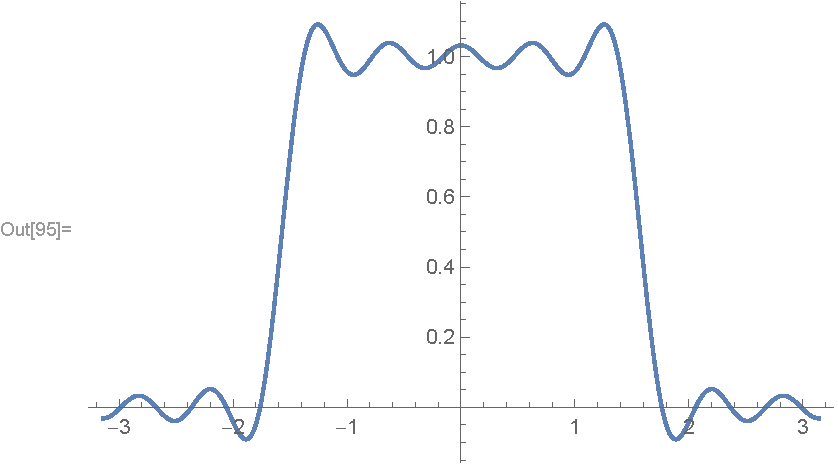
\includegraphics[width=\textwidth]{part3_plot1.pdf}
    \caption{$N=10$}

  \end{minipage}
  \hfill
  \begin{minipage}[b]{0.49\textwidth}
    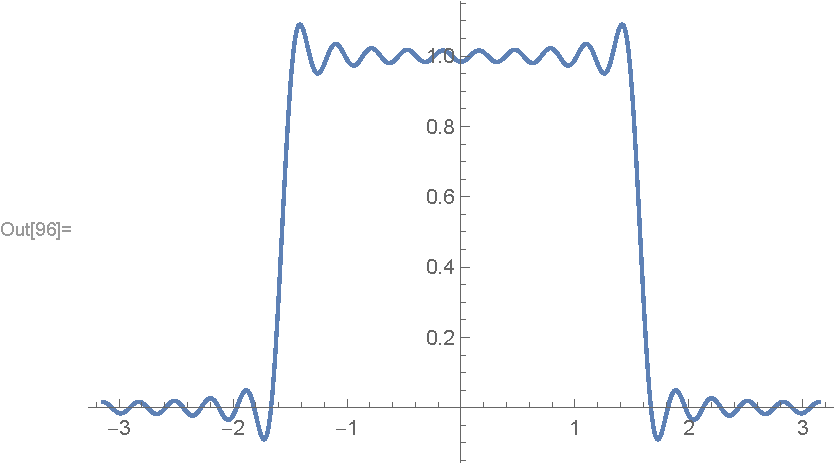
\includegraphics[width=\textwidth]{part3_plot2.pdf}
    \caption{$N=20$}

  \end{minipage}
    \hfill
  \begin{minipage}[b]{0.49\textwidth}
    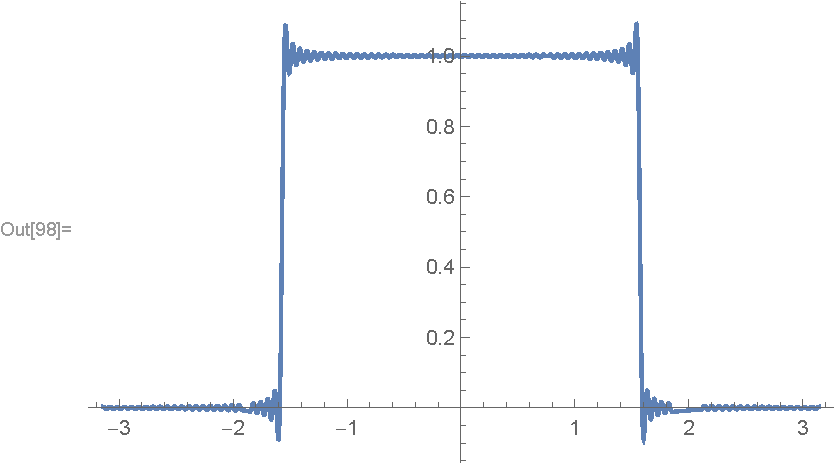
\includegraphics[width=\textwidth]{part3_plot3.pdf}
    \caption{$N=100$}

  \end{minipage}
    \hfill
  \begin{minipage}[b]{0.49\textwidth}
    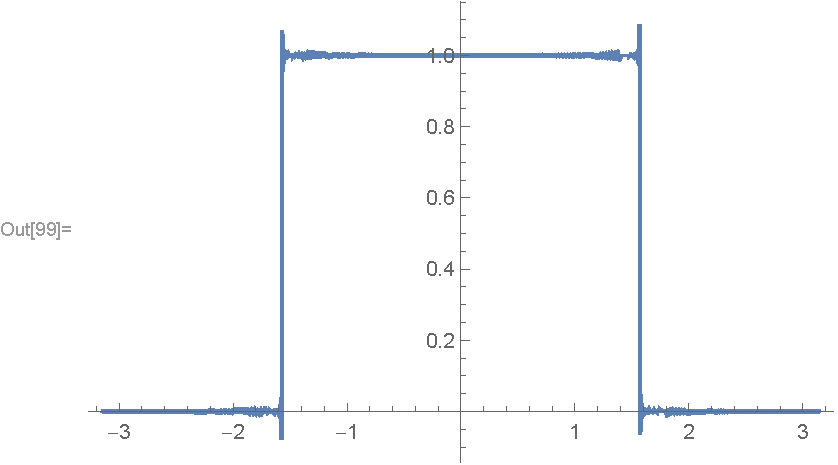
\includegraphics[width=\textwidth]{part3_plot4.pdf}
    \caption{$N=1000$}

  \end{minipage}
\end{figure}
\end{document}